%----------------------------------------------------------------------------
\chapter{\SystemDesign}
%----------------------------------------------------------------------------

%----------------------------------------------------------------------------
\section{Követelmények}
%----------------------------------------------------------------------------






 

%----------------------------------------------------------------------------
\section{Rendszerterv}
%----------------------------------------------------------------------------








!!!ÁBRA HELYE!!!
Egy jel útja a régi hibrid rendszerben





!!!ÁBRA HELYE!!!
Egy jel útja az új teljesen digitális rendszerben

%----------------------------------------------------------------------------
\subsection{Martin Audio Wavefront Precision hangrendszer}
%----------------------------------------------------------------------------



%----------------------------------------------------------------------------
\subsection{Allen \& Heath digitális keverőrendszer}
%----------------------------------------------------------------------------



%----------------------------------------------------------------------------
\subsection{Shure ULXD digitális vezeték nélküli mikrofonrendszer}
%----------------------------------------------------------------------------



%----------------------------------------------------------------------------
\subsection{Dante audio szerver}
%----------------------------------------------------------------------------



%----------------------------------------------------------------------------
\subsection{Dante hálózat kialakítása és optimalizálása}
%----------------------------------------------------------------------------

\subsubsection{Dante Controller: Hálózati mátrix}

Ezen a felületen tudjuk a hálózaton összekapcsolni a különböző hang vevőket és
adókat. Egy nagyobb rendszerben a konfigurálása rendkívül nagy odafigyelést és
precíziót igényel, pontosan tudnunk kell mit, hogyan és miért kötünk össze.

\subsubsection{Dante Controller: Eszköz nézet}

Lehetőségünk van két fő mód közül választani, a „redundant'' és a
„switched'' mód közül. A redundant mód mint ahogy azt a neve is sugallja
redundáns kommunikációt valósít meg az eszközök között szoftveresen és
hardveresen egyaránt, mivel az összes Dante kártya gyárilag két RJ45-s
csatlakozóval rendelkezik (jelen esetben ezt a módot választjuk az
üzembiztosság miatt) 
A másik lehetőség a switched pedig eszközök láncolását
teszi egyszerűbbé, így ha a rendundancia nem elsődleges szempont, nem kell
minden egyes eszköz mögé és switch, hanem a másodlagos RJ45 port direktbe köti
az arra csatlakoztatott eszközt az elsődleges hálózatra. A rendszer képes
automatikusan IP címeket osztani az egyes eszközöknek, így meggyorsítva a
munkafolyamatot. Egy fixen előre megtervezett rendszernél praktikusabb és
üzembiztosabb megoldás, ha minden eszköznek manuálisan megadjuk a címét a
hálózaton. A tervezett rendszerben minden egyes eszköznek fix IP címet adtam,
hogy a hálózat könnyebben és logikusan átlátható legyen az előbb említett előnyön kívül.
A címeket egy online is elérhető Excel táblázatban tároltam, hogy amennyiben szükség van rá
bármikor könnyen elérhető legyen.


\begin{figure}[!ht]
\centering
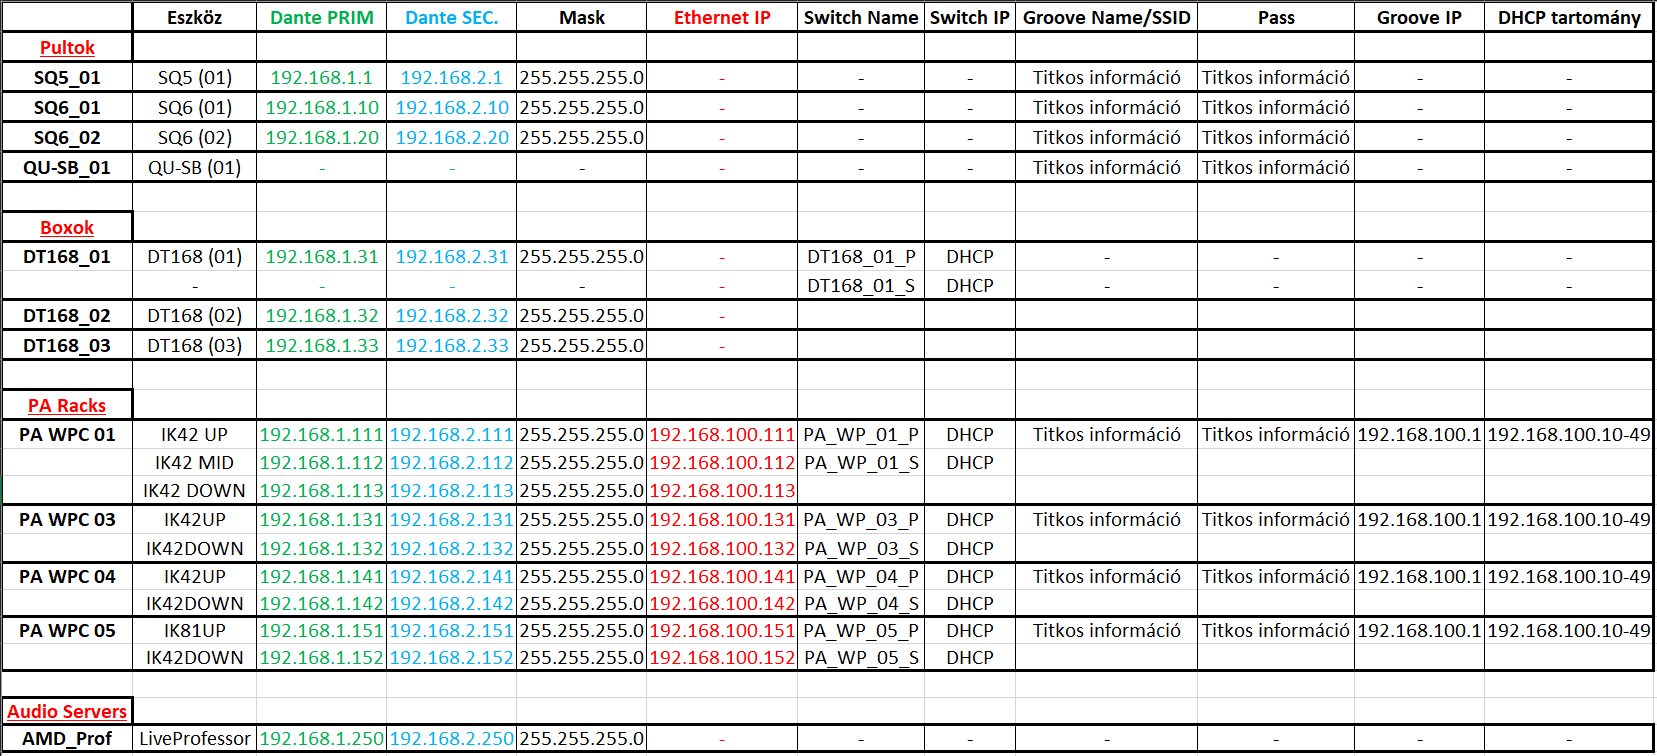
\includegraphics[width=150mm, keepaspectratio]{figures/Dante_IPs.png}
\caption{Dante eszközök IP címei a hálózaton}
\label{fig:Dante_IPs}
\end{figure}








\subsubsection{Dante Controller: Órajel nézet}

Meg kell adnunk az audio hálózatunk master órajelét, ehhez az órajelhez
szinkronizál a többi eszköz, az időszinkronizáció kulcsontosságú élőzenei
produkcióknál.



%----------------------------------------------------------------------------
\section{Rendszermérések és monitorozás}
%----------------------------------------------------------------------------



\subsubsection{Dante Controller: Hálózati állapot nézet}


\subsubsection{Dante Controller: Események nézet}





%----------------------------------------------------------------------------
\subsection{Cardioid mélyláda rendszer mérése}
%----------------------------------------------------------------------------



%----------------------------------------------------------------------------
\subsection{Mélyláda és Line Array fázishelyesség}
%----------------------------------------------------------------------------



%----------------------------------------------------------------------------
\subsection{Rendszer hangnyomás szint és frekvencia átvitel mérése}
%----------------------------------------------------------------------------



%----------------------------------------------------------------------------
\subsection{Dante rendszer monitorozása}
%----------------------------------------------------------------------------




